\frame{
%\begin{figure}[t]
%	\flushleft
%		\includegraphics[scale=0.1]{logo.jpg}
%\end{figure}

\begin{block}
{\begin{center} Quiz: Bolstapelprobleem van Kepler \end{center}}
\end{block}

\begin{figure}[h]
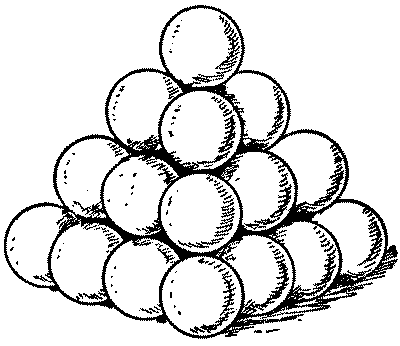
\includegraphics[width=4cm]{cannonballs}
\end{figure}
}
\section{Ontstaan}
\subsection{Vraag 1}
\begin{frame}

\begin{block}
{Wie was de wetenschappelijk adviseur van Sir Walter Raleigh?}

\begin{itemize}
	\item[A] Thomas Harriot
	\item[B] Johannes Kepler
	\item[C] Hij had geen wetenschappelijk adviseur
\end{itemize}
\end{block}

\begin{figure}
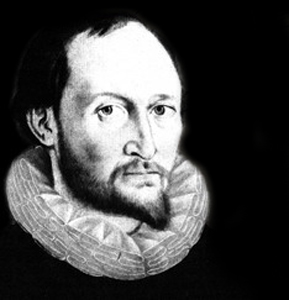
\includegraphics[height=3cm]{harriot}
\end{figure}


\end{frame}

\begin{frame}

\begin{block}
{Wie was de wetenschappelijk adviseur van Sir Walter Raleigh?}

\begin{itemize}
	\item[\textbf{A}] \textbf{Thomas Harriot}
	\item[B] Johannes Kepler
	\item[C] Hij had geen wetenschappelijk adviseur
\end{itemize}
\end{block}

\begin{figure}
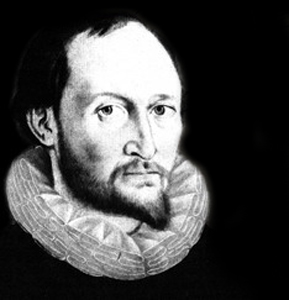
\includegraphics[height=3cm]{harriot}
\end{figure}


\end{frame}

\subsection{Vraag 2}

\begin{frame}

\begin{block}
{Wat is de nationaliteit van Johannes Kepler?}

\begin{itemize}
	\item[A] Duitser
	\item[B] Oostenrijker
	\item[C] Engelsman
	\end{itemize}
\end{block}
\begin{figure}[h]
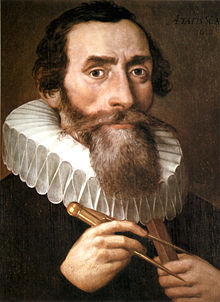
\includegraphics[heigth=5cm]{kepler}

\end{figure}

\end{frame}


\begin{frame}

\begin{block}
{Wat is de nationaliteit van Johannes Kepler?}

\begin{itemize}
	\item[\textbf{A}] \textbf{Duitser}
	\item[B] Oostenrijker
	\item[C] Engelsman
	\end{itemize}
\end{block}
\begin{figure}[h]
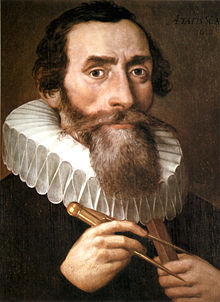
\includegraphics[heigth=5cm]{kepler}

\end{figure}

\end{frame}


\subsection{Vraag 3}
\begin{frame}

\begin{block}
{Welke term betekent niet 'het maximum aantal niet-overlappende eenheidssferen dat aan een gegeven eenheidssfeer raakt'?}

\begin{itemize}
	\item[A] Newton number
	\item[B] Kissing number
	\item[C] Contact number
	\item[D] Kepler number
	\end{itemize}
\end{block}

\begin{figure}[h]
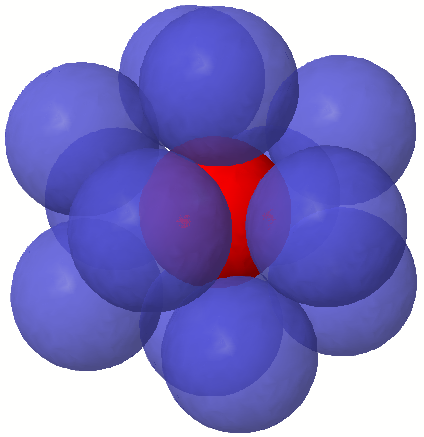
\includegraphics[width=3cm]{kissing}
\end{figure}
%D

\end{frame}

\begin{frame}

\begin{block}
{Welke term betekent niet 'het maximum aantal niet-overlappende eenheidssferen dat aan een gegeven eenheidssfeer raakt'?}

\begin{itemize}
	\item[A] Newton number
	\item[B] Kissing number
	\item[C] Contact number
	\item[\textbf{D}] \textbf{Keper number}
	\end{itemize}
\end{block}

\begin{figure}[h]
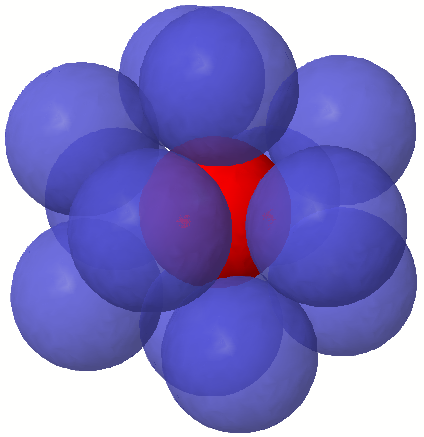
\includegraphics[width=3cm]{kissing}
\end{figure}
%D

\end{frame}


\section{Evolutie}
\subsection{Vraag 4}

\begin{frame}

\begin{block}{Welke Duitse Wiskundige bewees dat de \textquoteleft face-centered cubic packing' de dichtste pakkingsmethode is volgens een rooster?}
\begin{itemize}
	\item[A] Kepler
	\item[B] Gauss
	\item[C] Hilbert 
\end{itemize}
\end{block}

\begin{figure}[h]
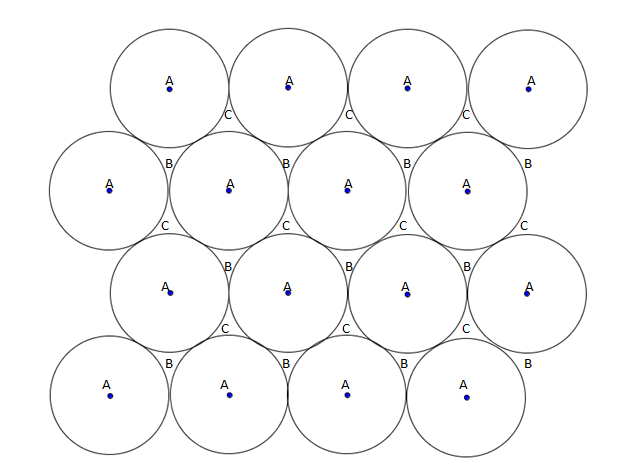
\includegraphics[height=3cm]{fcc}
\end{figure}
\end{frame}

\begin{frame}

\begin{block}{Welke Duitse Wiskundige bewees dat de \textquoteleft face-centered cubic packing' de dichtste pakkingsmethode is volgens een rooster?}
\begin{itemize}
	\item[A] Kepler
	\item[\textbf{B}] \textbf{Gauss}
	\item[C] Hilbert 
\end{itemize}
\end{block}

\begin{figure}[h]
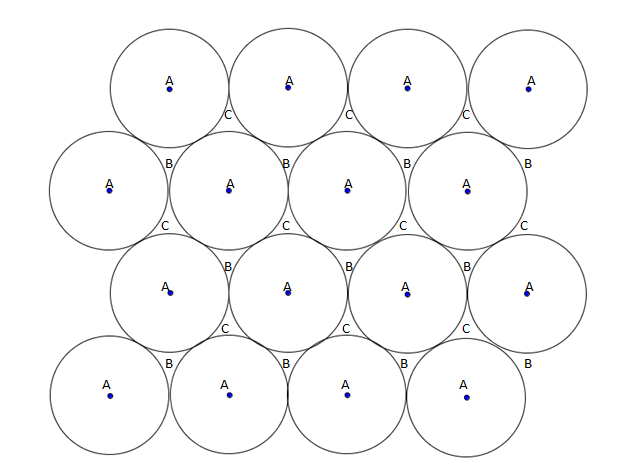
\includegraphics[height=3cm]{fcc}
\end{figure}
\end{frame}


\subsection{Vraag 5}

\begin{frame}
\begin{block}
{Welke Scandinavische wiskundige ontwikkelde een theorie over het tweedimensionale equivalent voor 'het probleem van Kepler' waarin men zicht naar de dichtste pakkingsmethode voor cirkels in het vlak?}
\begin{itemize}
	\item[A] Axel Thue
	\item[B] L�szlo Feje T�th
	\item[C] Wu-Yi Hsiang
	\end{itemize}
\end{block}
\begin{figure}[h]
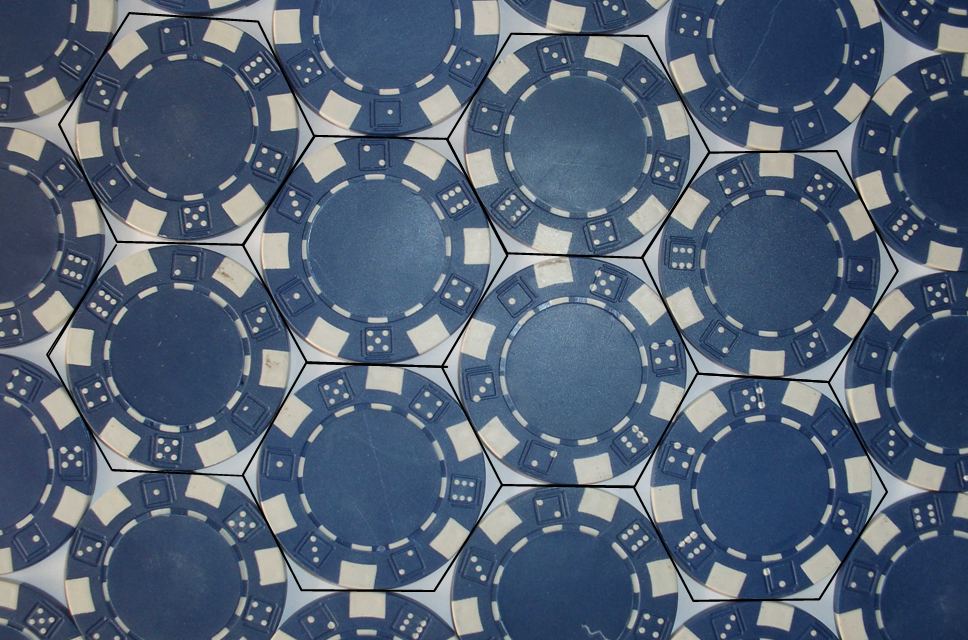
\includegraphics[width=3cm]{voronoi_hex}
\end{figure}
\end{frame}

\begin{frame}
\begin{block}
{Welke Scandinavische wiskundige ontwikkelde een theorie over het tweedimensionale equivalent voor 'het probleem van Kepler' waarin men zicht naar de dichtste pakkingsmethode voor cirkels in het vlak?}

\begin{itemize}
	\item[\textbf{A}] \textbf{Axel Thue}
	\item[B] L�szlo Feje T�th
	\item[C] Wu-Yi Hsiang
	\end{itemize}
\end{block}

\begin{figure}[h]
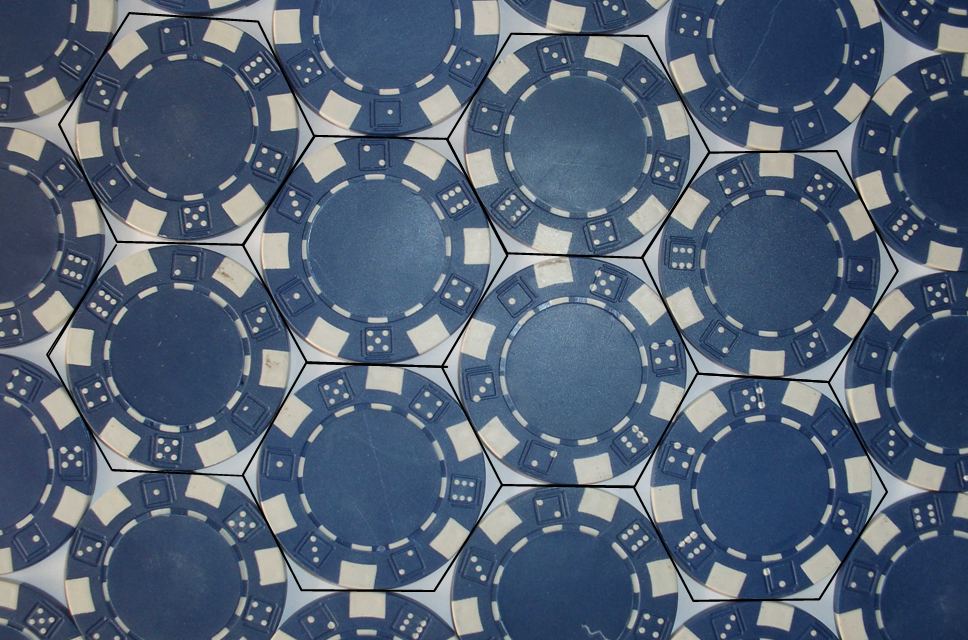
\includegraphics[width=3cm]{voronoi_hex}
\end{figure}

\end{frame}

\subsection{Vraag 6}

\begin{frame}
\begin{block}
{Kepler vermoedde dat de dichtheid van de dichtste bolstapeling $\frac{\pi}{\sqrt{18}}$ is. Wat is deze effici�ntie als percentage?}

\begin{itemize}
	\item[A] 74,0480 \%
	\item[B] 77,964 \%
	\item[C] 77,844 \%
	\item[D] 77,3055 \%
	\end{itemize}
\end{block}


\end{frame}


\begin{frame}
\begin{block}
{Kepler vermoedde dat de dichtheid van de dichtste bolstapeling $\frac{\pi}{\sqrt{18}}$ is. Wat is deze effici�ntie als percentage?}

\begin{itemize}
	\item[\textbf{A}] \textbf{74,0480 \%}
	\item[B] 77,964 \%
	\item[C] 77,844 \%
	\item[D] 77,3055 \%
	\end{itemize}
\end{block}

\end{frame}
\section{Bewijs}
\subsection{Vraag 7}

\begin{frame}
\begin{block}
{Voor hoeveel stapelingen moest Thomas Hales uiteindelijk het probleem van Kepler aantonen?}

\begin{itemize}
	\item[A] 5
	\item[B] 50
	\item[C] 500
	\item[D] 5000
	\end{itemize}
\end{block}

\begin{figure}[h]
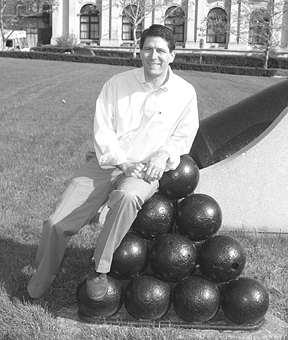
\includegraphics[width=3cm]{hales}
\end{figure}

\end{frame}


\begin{frame}
\begin{block}
{Voor hoeveel stapelingen moest Thomas Hales uiteindelijk het probleem van Kepler aantonen?}

\begin{itemize}
	\item[A] 5
	\item[B] 50
	\item[C] 500
	\item[\textbf{D}] \textbf{5000}
	\end{itemize}
\end{block}

\begin{figure}[h]
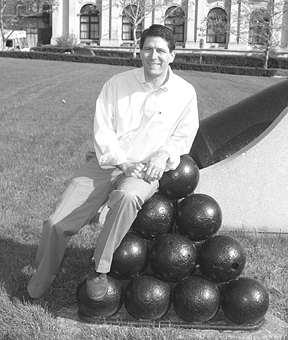
\includegraphics[width=3cm]{hales}
\end{figure}

\end{frame}

\subsection{Vraag 8}

\begin{frame}
\begin{block}
{Waarom bleken er voor sommigen achteraf nog twijfels over het bewijs van Hales ?}

\begin{itemize}
	\item[A] Eigenlijk was het zijn assistent Samuel Ferguson die het bewijs had geleverd.
	\item[B] Het bewijs is zo lang dat het niet gecontroleerd kan worden.
	\item[C] Hales bewees de stelling met de computer.
	\end{itemize}
\end{block}

\begin{figure}[h]
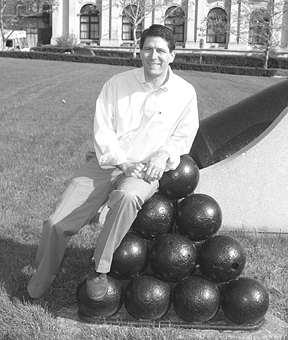
\includegraphics[width=3cm]{hales}
\end{figure}

\end{frame}


\begin{frame}
\begin{block}
{Waarom bleken er voor sommigen achteraf nog twijfels over het bewijs van Hales ?}

\begin{itemize}
	\item[A] Eigenlijk was het zijn assistent Samuel Ferguson die het bewijs had geleverd.
	\item[B] Het bewijs is zo lang dat het niet gecontroleerd kan worden.
	\item[\textbf{C}] \textbf{Hales bewees de stelling met de computer.}
	\end{itemize}
\end{block}

\begin{figure}[h]
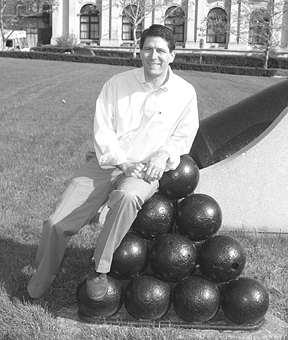
\includegraphics[width=3cm]{hales}
\end{figure}

\end{frame}

